\section{Auswertung}

\subsection{Berechnung des mittleren Verschiebungsquadrates und dessen Fehler}

Wir betrachten zunächst den Weg unseres ausgewählten Partikels in der zweidimensionalen Ebene, zu sehen in \abbref{fig:brown1}. Es ist zu beachten, dass das Partikel durch auch Bewegungen in der vertikalen $z$-Ebene ausgeführt hat. Dies haben wir hier vernachlässigt, was zu einem späteren Zeitpunkt auch bei der Fehlerdiskussion relevant ist.


\begin{figure}[H]
  \centering
  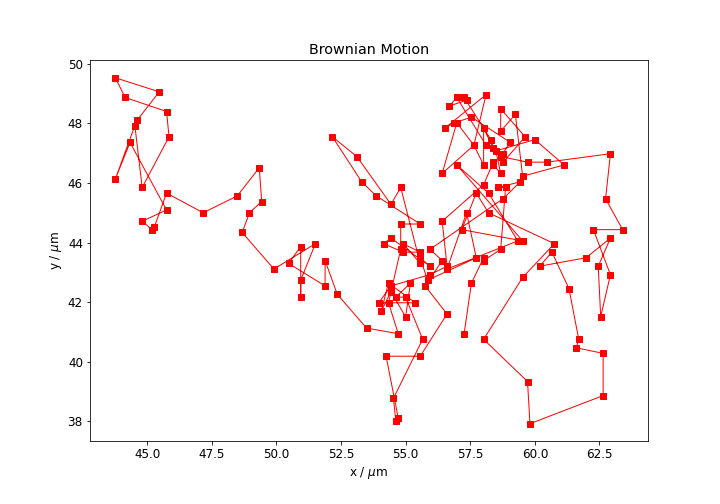
\includegraphics[width=.90\textwidth]{files/brown1.png}
  \caption{Aufgezeichneter Weg des Partikels in der zweidimensionalen Ebene.}
  \label{fig:brown1}
\end{figure}

Aus der Änderung zweier nebeneinander liegender $x$- und $y$-Koordinaten
\begin{gather}
  \Delta x_i = x_{i+1} - x_i\\
  \Delta y_i = y_{i+1} - y_i
\end{gather}
berechnen wir nun die mittleren Verschiebungsquadrate $\expval{x^2}$ und $\expval{y^2}$ in $x$- bzw. $y$-Richtung. Sowie daraus das gesamte mittlere Verschiebungsquadrat $\expval{r^2}$ nach Gleichung \eqref{eq:r_squared}. Als Mittelwert über alle Verschiebungsquadrate zwischen je zwei nebeneinander liegenden aufgezeichneten Koordinaten kommen wir damit auf
\begin{align}
  \overline{\expval{r^2}} = (2.12 \pm 0.18) \cdot 10^{-12} \si{\meter}.
\end{align}

Der mittlere zeitliche Abstand zwischen zwei Koordinatenaufzeichnugen beträgt jeweils $\overline{t} = 1\si{\second}$.

Nach Gleichung \eqref{eq:k_boltz} können wir nun einen Wert für die Boltzmannkonstante berechnen. Hierzu ziehen wir noch die Daten aus dem Messprotokoll hinzu Teilchendurchmesser $(755 \pm 30)\si{\nano\meter}$, diesen rechnen wir noch in den Radius $a$ um, sowie die Zimmertemperatur $T = (22.2 + 274.15 \pm 0.1)  \si{\kelvin}$. Wir erhalten einen Wert von
\begin{align}
  k_{B,1} = (1.21 \pm  0.12) \cdot 10^{-23}.
\end{align}
Aufgrund der großen Anzahl an Variablen in dieser Formel verwenden wir hier für die Fehlerberechnung die relativen Fehler:
\begin{align}
  \Delta k_{B,1} = k_{B,1} \cdot \sqrt{\relerrsq{\overline{\expval{r^2}}} + \relerrsq{a} + \relerrsq{\eta_{H_2 O}} + \relerrsq{T} + \relerrsq{t}}.
\end{align}

Um den Diffusionskoeffizienten $D$ zu berechnen stellen wir die Gleichung $\sqrt{\expval{r^2}} = \sqrt{4Dt}$ um, zu
\begin{gather}
  D = \frac{1}{4} \frac{\overline{\expval{r^2}}}{\overline{t}}
  \intertext{und erhalten}
  D = (5.3 \pm 0.5) \cdot 10^{-13}
\end{gather}
mit Fehler nach der klassischen Gauß'schen Fehlerfortpflanzung.

\subsection{Kontrollverteilung}

Wir möchten nun die mathematische Aussage prüfen, dass die Wahrscheinlichkeit, ein Partikel nach der Zeit $t$ im Intervall $\qty[x, x + \Delta x]$ befindet tatsächlich einer Gaussverteilung folgt. Hierzu fügen wir alle berechneten mittleren Verschiebungsquadrate in $x$- und $y$-Richtung in eine gemeinsame Liste und stellen die Werte in einem Histogramm, siehe \abbref{fig:brown2}, dar.

\begin{figure}[H]
  \centering
  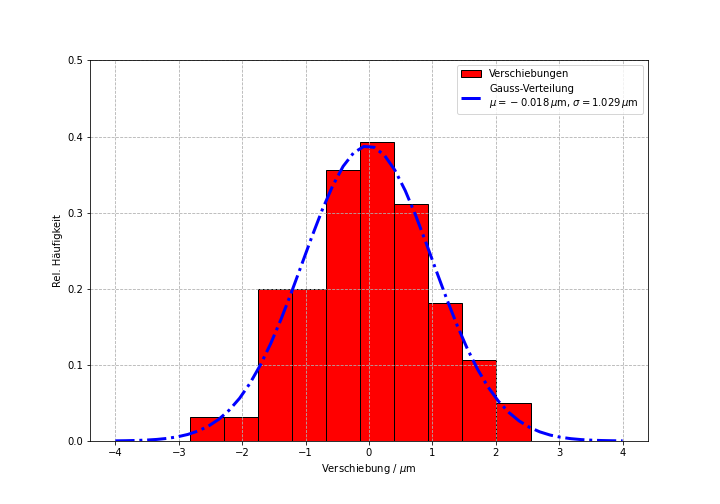
\includegraphics[width=.90\textwidth]{files/brown2.png}
  \caption{Histogramm der mittleren Verschiebungsquadrate in in $x$- und $y$-Richtung.}
  \label{fig:brown2}
\end{figure}

$\mu$ und $\sigma^2$ der im Plot in blau dargestellten Gaußkurve berechnen wir aus den Daten anhand der standardmäßigen Formeln für Mittelwert und Standardabweichung
\begin{gather}
  \mu = \frac{1}{N} \sum_{i = 1}^N x_i,\\
  \sigma = \sqrt{\frac{1}{N} \sum_{i = 1}^N \qty|x_i - \overline{x}|^2}.
\end{gather}

Es ist gut zu erkennen, dass die Kurve die Form der Daten bereits sehr gut beschreibt.

\subsection{Kumulative Verteilung der Verschiebungsquadrate}

Für einen weiteren Ansatz zur Berechnung der Boltzmannkonstante betrachten wir nun zunächst die kumulative Verschiebung als Funktion der Zeit, also deren kumulative Verteilung, dargestellt in \abbref{fig:brown3}.

\begin{figure}[H]
  \centering
  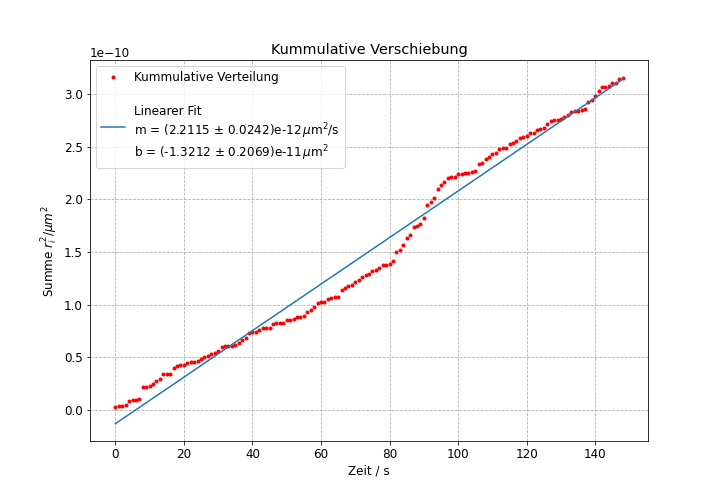
\includegraphics[width=.90\textwidth]{files/brown3.png}
  \caption{Kumulative Verschiebung eines Partikels als Funktion der Zeit.}
  \label{fig:brown3}
\end{figure}

An die Verteilung fitten wir eine standardmäßige lineare Funktion der Form $mx + b$, im Plot dargestellt in Blau. Die optimierten Werte für $m$ und $b$, sowie deren Fehler, sind in der Legende des Plots angegeben. Mit der Steigung $m$ der Geraden können wir nun das Verhältnis $\frac{\overline{\expval{r^2}}}{\overline{t}}$ in der ursprünglichen Formel für die Boltzmannkonstante ersetzen. Es gilt also
\begin{gather}
  k_{B,2} = \frac{6\pi\eta a m}{4 T}\\
  \intertext{und}
  \Delta k_{B,2} = k_{B,2} \cdot \sqrt{\relerrsq{m} + \relerrsq{a} + \relerrsq{\eta_{H_2 O}} + \relerrsq{T}}.
\end{gather}

Wir berechnen damit einen Wert von
\begin{align}
  k_{B,2} = (1.26 \pm 0.06) \cdot 10^{-23}.
\end{align}

Die Formel für den Diffusionskoeffizienten reduziert unter Verwendung der Steigung $m$ auf
\begin{align}
  D = \frac{1}{4} m = (5.53 \pm 0.07) \cdot 10^{-13}.
\end{align}